\documentclass[tikz,border=10pt]{standalone}
% Only the TikZ libraries needed here: none beyond the core
\begin{document}
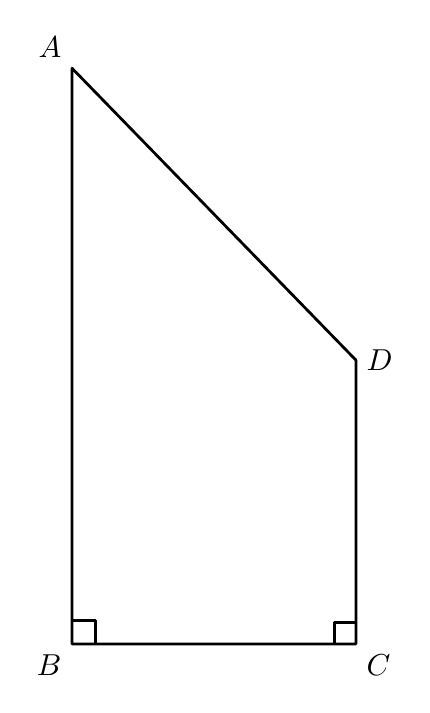
\begin{tikzpicture}[line width=1.0pt, line join=round]
  % Scale s = 0.012739 cm/px, centre = ink bbox centre (212.5, 349) px, y flipped
  \coordinate (A) at (-1.8281,  3.7070);
  \coordinate (B) at (-1.8281, -3.6049);
  \coordinate (C) at ( 1.7773, -3.6049);
  \coordinate (D) at ( 1.7773,  0.0000);

  % Quadrilateral ABCD (solid edges)
  \draw (A) -- (B) -- (C) -- (D) -- cycle;

  % Right-angle mark at B (0.2967 cm square, from mark_points_px)
  \draw (-1.8281,-3.3082) -- (-1.5314,-3.3082) -- (-1.5314,-3.6049);

  % Right-angle mark at C (0.2708 cm square, from mark_points_px)
  \draw ( 1.7773,-3.3341) -- ( 1.5065,-3.3341) -- ( 1.5065,-3.6049);

  % Vertex labels (math mode, outside the figure)
  \node[above left]  at (A) [font=\fontsize{10.5}{12.6}\selectfont] {$A$};
  \node[below left]  at (B) [font=\fontsize{10.5}{12.6}\selectfont] {$B$};
  \node[below right] at (C) [font=\fontsize{10.5}{12.6}\selectfont] {$C$};
  \node[right]       at (D) [font=\fontsize{10.5}{12.6}\selectfont] {$D$};
\end{tikzpicture}
\end{document}